%--------------------------------------------------------------------------------------------------
\section{Cross Attention Stream}
\begin{figure*}[t]
    \centering
    \begin{tikzpicture}[
        font={\footnotesize},
        trap/.style={trapezium, rotate=-90,trapezium angle=75},
    ]
        %% CNN branch
        \node(input) at (-5.5, 0) {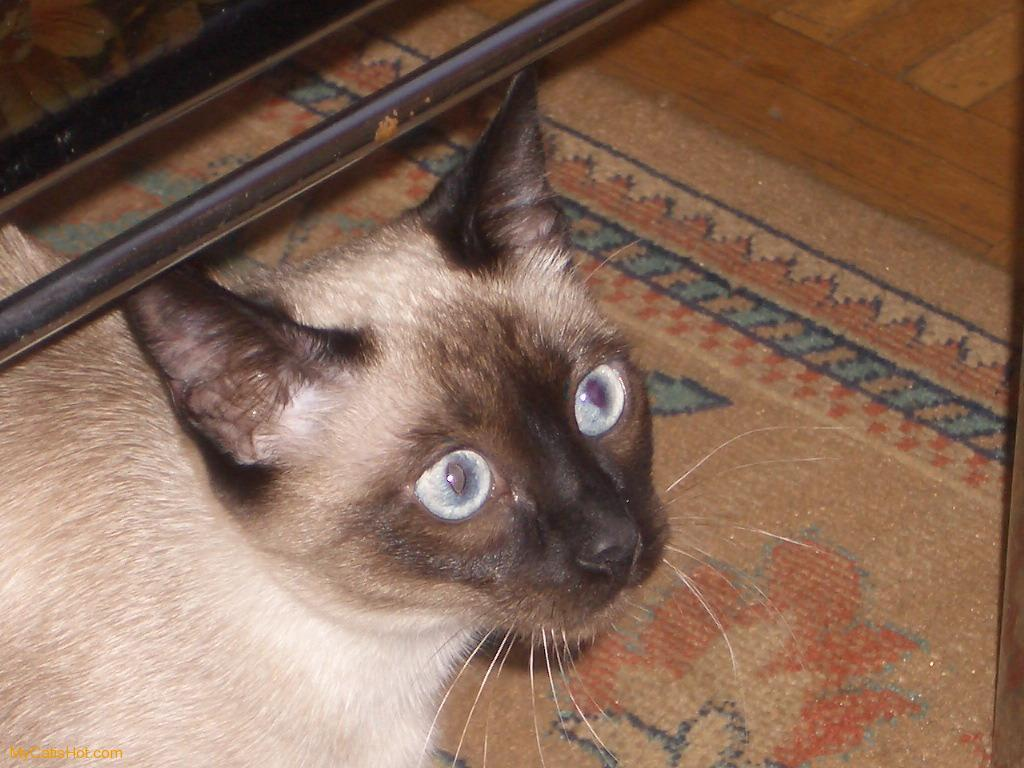
\includegraphics[width=.1\textwidth]{Images/Method/input.jpg}};
        \node[above] at (input.north) {Input image $\vx$};
        \node[draw, trap] (res0) at (-3.5,0) {\rotatebox{90}{\parbox{1.0cm}{\centering{Res-0}}}};
        \node[draw, trap] (res1) at (-1.5,0) {\rotatebox{90}{\parbox{1.0cm}{\centering{Res-1}}}};
        \node[draw, trap] (res2) at (0.5,0) {\rotatebox{90}{\parbox{1.0cm}{\centering{Res-2}}}};
        \node[draw, trap] (res3) at (2.5,0) {\rotatebox{90}{\parbox{1.0cm}{\centering{Res-3}}}};
        \node[draw, trap] (res4) at (4.5,0) {\rotatebox{90}{\parbox{1.0cm}{\centering{Res-4}}}};
        \node[](empt1) at (6.75, 0){};
        \node[draw, rotate=90, align=center] (class) at (7.5,0) {Classifier};
        \node(logit) at (8.25, 0) {$\vy$};
        %%% CLS stream
        \node[](clsin) at (-4, -1.5) {{$\vq_0$}};
        \node[draw](CA0) at (-2.5, -1.5) {{CA-0}};
        \node[draw](CA1) at (-0.5, -1.5) {{CA-1}};
        \node[draw](CA2) at (1.5, -1.5)  {{CA-2}};
        \node[draw](CA3) at (3.5, -1.5)  {{CA-3}};
        \node[draw](CA4) at (5.5, -1.5)  {{CA-4}};
    
        %% CNN backbone
        \node(empt0) at (-4.65, 0) {};
        \draw[->] (empt0.center) -- node {} (res0);
        \draw[->] (res0) -- node[above] {$F_0$} (res1);
        \draw[->] (res1) -- node[above] {$F_1$} (res2);
        \draw[->] (res2) -- node[above] {$F_2$} (res3);
        \draw[->] (res3) -- node[above] {$F_3$} (res4);
        \draw[->, blue, dashed] (res4) -- node {\blue{\normalsize//}} (class);
        \node[](GAP) at (6.25,0.25) {\blue{$\gap$}};
        \draw[->] (class) -- node {} (logit);
        %% CLS Stream
        \draw[->] (clsin) -- node {} (CA0);
        \draw[dashed, ->] (res0.north) -|node {} (CA0);
        \draw[->] (CA0) -- node[above] {$\vq_1$} (CA1);
        \draw[dashed, ->] (res1.north) -|node {} (CA1);
        \draw[->] (CA1) -- node[above] {$\vq_2$} (CA2);
        \draw[dashed, ->] (res2.north) -|node {} (CA2);
        \draw[->] (CA2) -- node[above] {$\vq_3$} (CA3);
        \draw[dashed, ->] (res3.north) -|node {} (CA3);
        \draw[->] (CA3) -- node[above] {$\vq_4$} (CA4);
        \draw[dashed, ->] (res4.north) -|node[above] {$F_4$} (CA4);
        \draw[-] (CA4.east) -| node[right] {$\vq_5$} (empt1.center);
        \draw[->] (empt1.center) -- node {} (class);
    \end{tikzpicture}
    \vspace{3pt}
    \caption{\emph{\OURS (\Ours) applied to ResNet-based architectures.} Given a network $f$, we replace global average pooling (\gap) by a learned, attention-based pooling mechanism implemented as a stream in parallel to $f$. The feature tensor $F_\ell \in \real^{p_\ell \times d_\ell}$ (\emph{key}) obtained by stage Res-$\ell$ of $f$ interacts with a \cls token (\emph{query}) embedding $\vq_\ell \in \real^{d_\ell}$ in block CA-$\ell$, which contains cross attention~\eq{CA} followed by a linear projection~\eq{qk-layer} to adapt to the dimension of $F_{\ell+1}$. Here, $p_\ell$ is the number of patches (spatial resolution) and $d_\ell$ the embedding dimension. The query is initialized by a learnable parameter $\vq_0 \in \real^{d_0}$, while the output $\vq_5$ of the last cross attention block is used as a global image representation into the classifier. The network and classifier are pretrained and kept frozen while the parameters of \Ours are learned. At inference, we use existing post-hoc interpretability methods like Grad-CAM~\citep{DBLP:journals/corr/SelvarajuDVCPB16} to obtain saliency maps for both the baseline \gap and our \Ours. We compare interpretability metrics as well as accuracy.}
    \label{fig:fig_method}
    \end{figure*}
    
\label{sec:ca_design}
Motivated by the observations above, we design a \emph{\OURS} (\emph{\Ours}) in parallel to any 
network. It takes input features at key locations of the network and uses cross attention to build 
a global image representation and replace $\gap$ before the classifier. An example is shown in 
\autoref{fig:fig_method}, applied to a ResNet-based architecture.

\paragraph{Architecture}
More formally, given a network $f$, we consider points between blocks of $f$ where critical 
operations take place, such as change of spatial resolution or embedding dimension, \eg between 
stages for ResNet. We decompose $f$ at these points as
\begin{equation}
	f = g \circ \gap \circ f_L \circ \dots \circ f_0
\label{eq:f-decomp}
\end{equation}
such that features $F_\ell \in \real^{p_\ell \times d_\ell}$ of layer (stage) $\ell$ are 
initialized as $F_{-1} = \vx$ and updated according to

\begin{equation}
	F_\ell = f_\ell(F_{\ell-1})
\label{eq:f-layer}
\end{equation}
for $0 \le \ell \le L$. The last layer features $F_L$ are followed by \gap and $g: \real^{d_L} \to 
\real^C$ is the classifier, mapping to the logit vector $\vy$. As in ~\eq{sal}, 
$p_\ell$ is the number of patch tokens and $d_\ell$ the embedding dimension of stage $\ell$.

In parallel, we initialize a classification token embedding as a learnable parameter $\vq_0 \in 
\real^{d_0}$ and we build a sequence of updated embeddings $\vq_\ell \in \real^{d_\ell}$ along a 
stream that interacts with $F_\ell$ at each stage $\ell$. Referring to the global representation 
$\vq_\ell$ as \emph{query} or \cls and to the local image features $F_\ell$ as \emph{key} or patch 
embeddings, the interaction consists of cross attention followed by a linear projection $W_\ell \in 
\real^{d_{\ell+1} \times d_\ell}$ to account for changes of embedding dimension between the 
corresponding stages of $f$:

\begin{equation}
	\vq_{\ell+1} = W_\ell \cdot \ca_\ell(\vq_\ell, F_\ell),
\label{eq:qk-layer}
\end{equation}
for $0 \le \ell \le L$, where $\ca_\ell$ is defined as in~\eq{CA}. 
% Because of linearity, projection $W_\ell$ is the same as a value projection.

Image features $F_0, \dots, F_L$ do not change by injecting our \Ours into network $f$. However, 
the final global image representation and hence the prediction do change. In particular, at the 
last stage $L$, $\vq_{L+1}$ is used as a global image representation for classification, 
replacing \gap over $F_L$. The final prediction is $g(\vq_{L+1}) \in \real^C$. Unlike \gap, the 
weights of different image patches in the linear combination are non-uniform, enhancing the 
contribution of relevant patches in the prediction.

%--------------------------------------------------------------------------------------------------
\paragraph{Training}

In this sense, the network $f$ is pretrained and remains frozen while we learn the parameters of 
our \Ours on the same training set as one used to train $f$. The classifier is kept frozen too. 
Referring to~\eq{f-decomp}, $f_0, \dots, f_L$ and $g$ are fixed, while \gap is replaced by learned 
weighted averaging, with the weights obtained by the \Ours.

\paragraph{Inference}
As it stands, \Ours is not an interpretability method, but rather a modification of the baseline 
architecture, \ie, an attention-based pooling mechanism that replaces \gap to enhance the 
contribution of relevant image regions in the prediction. We are interested in investigating the 
interpretability properties of this modification. We therefore employ existing post-hoc, CAM-based 
interpretability methods to generate saliency maps with both baseline \gap and \Ours. We then 
compare interpretability metrics as well as classification accuracy.